\chapter{Propozycja wykorzystania warstwy pośredniej}
\label{cha:middleware}

W rozdziale poprzednim  podczas analizy sposobu działania klienckich aplikacji mobilnych, wyciągnięto wniosek, że najbardziej odpowiednim miejscem do wykorzystania procesów biznesowych, będą aplikacje back end'owe. Stwierdzono również, że w celu realizacji takiego rozwiązania konieczne jest zastosowanie dodatkowej warstwy pośredniej, realizującej komunikacje aplikacji mobilnych z procesami biznesowymi. Głównym powodem stosowania warstwy pośredniej jest brak możliwości udostępnienia przez aplikacje mobilne, usług sieciowych z którymi proces mógłby się komunikować. 

\begin{figure}[h]
\centerline{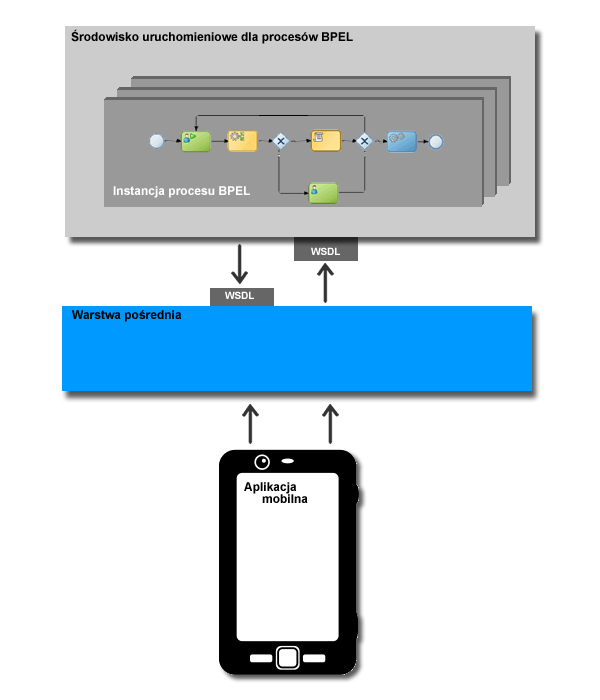
\includegraphics[scale=0.5]{middlewareConceptDiagram}}
\caption{Poglądowy schemat działania warstwy pośredniej}
\label{fig:middlewareConceptDiagram}
\end{figure}

Na rysunku~\ref{fig:middlewareConceptDiagram}. przedstawiono poglądowy schemat działania opisanego powyżej rozwiązania. Diagram ma na celu lepsze zobrazowanie problemu i wyłonienie funkcjonalności, które warstwa pośrednia musi realizować. Na schemacie można dostrzec trzy rodzaje systemów: środowisko uruchomieniowe dla procesów biznesowych, warstwę pośrednią oraz aplikację mobilną. Strzałki umieszczone na schemacie przedstawiają kierunki komunikacji pomiędzy poszczególnymi systemami.  Komunikacja między aplikacją mobilną a warstwą pośrednią zawsze odbywa się z inicjatywy aplikacji mobilnej, jest to związane ze specyfiką dostępu aplikacji do mediów komunikacyjnych. Wynika z tego, że jedną z funkcjonalności które musi  realizować warstwa pośrednia jest buforowanie żądań pochodzących z procesów biznesowych do momentu aż aplikacja mobilna się po nie zgłosi sama. 

Aplikacje mobilne są specyficzne pod jeszcze jednym względem - poszczególne instancje aplikacji uruchamiane są zawsze na urządzeniach personalnych. Bardzo mocny akcent zatem kładziony jest tutaj na samych użytkowników. Gdy przyglądniemy się procesowi BPEL to możemy dostrzec, że wątek ludzki jest w nich zupełnie pomijany. Proces komunikuje się z usługą sieciową jedynie w celu rozwiązania jakiegoś konkretnego zadania i zazwyczaj oczekuje na rezultat.

%---------------------------------------------------------------------------

\section{BPEL4People}
\label{sec:BPEL4People}

Jak wspomniano powyżej procesy WS-BPEL traktują użytkowników po macoszemu, skupiają się przede wszystkim na sekwencji wykonywania kolejnych operacji. Problem dostrzegli projektanci z zespołów IBM oraz SAP, a proponowaną przez nich odpowiedzią jest powstanie rozszerzenia do BPEL nazwanego \textit{BPEL4People}.  

Twórcy standardu argumentują powstanie kolejnej specyfikacji koniecznością uwzględnienia aspektu ludzkiego w procesach BPEL. Podają szereg przykładów, w których interakcja procesu z człowiekiem jest konieczna. Jednym z przykładów jest konieczność dokonywania decyzji akceptacji lub odrzucenia wyniku jakiejś operacji. Innym przykładem jest wprowadzanie dodatkowych danych niezbędnych do kontynuacji wykonania procesu, za pomocą formularzy\cite[str. 4]{bpel4People}.

Specyfikacja opiewa w szereg bardzo ciekawych pomysłów integracji interakcji użytkowników z  procesami BPEL. Porusza problem przejścia pomiędzy serwisami dostosowanymi dla ludzi a serwisami zautomatyzowanymi, zwraca uwagę na  problem monitorowania zadań przeznaczonych dla ludzi, opisuje problem terminów ostatecznych wykonania zadań oraz eskalacji w przypadku ich przekroczenia\cite[str. 6]{bpel4People}.

\subsection{WS-HumanTask}

Bezpośrednio powiązany  z rozszerzeniem \textit{BPEL4people} jest temat usług sieciowych dla ludzi, które są wykorzystywane przez to rozszerzenie.

\textit{WS-HumanTask} są usługami sieciowymi 'implementowanymi' przez ludzi. Pozwalają na integrację ludzi z aplikacjami zorientowanymi na usługi (SOA). Specyfikacja udostępnia dwa interfejsy do komunikacjami z zadaniami. Pierwszy z nich jest przeznaczony dla automatów czyli aplikacji rozproszonych, drugi natomiast jest przeznaczony dla ludzi i pozwala na operacje zadaniami.  
Zadania opisane w specyfikacji posiadają przypisania do konkretnych grup docelowych. Przypisania te definiują kto powinien być uprawniony do operacji na zadaniach. Specyfikacja definiuje również meta dane dotyczące zadań, pozwalające na określenie w jaki sposób zadania mają być prezentowane na różnych urządzeniach. Zadanie mogą również definiować reakcje na terminy ostateczne ich wykonania, w postaci mechanizmu eskalacji. 

\subsection{Implementacje}

Z punku widzenia proponowanego w niniejszej pracy magisterskiej rozwiązanie zastosowanie \textit{BPEL4People} rozwiązuje szereg problemów związanych ze spersonalizowaną specyfiką aplikacji mobilnych. Kolejne instancje aplikacji mobilnych można utożsami z użytkownikami. Warstwa pośrednia udostępniałaby w takim podejściu WS-HT, z którymi komunikowałby się proces \textit{BPEL4People}. Niestety rzeczywistość w tym przypadku okazuje się brutalna. Rozszerzenie do BPEL jeśli nie zostaje zaimplementowane jest bezwartościowe. W przypadku \textit{BPEL4People} mimo tego że standard istnieje już 9 lat, nie został jeszcze wdrożony w żadnym z popularnych środowisk uruchomieniowych.  
Warstwa pośrednia powinna więc, samodzielnie uwzględniać aspekt ludzki pomijany przez procesy WS-BPEL. 

Mimo braku implementacji można dostrzec pewne korzyści płynące z powstania rozszerzenia BPEL4People. Są nimi z pewnością pomysły dotyczące rozwiązania problemu dystrybucji żądań pochodzących z procesów WS-BPEL między różnymi użytkownikami. W niniejszej pracy magisterskiej niejednokrotnie skorzystamy z tej wiedzy. 

%---------------------------------------------------------------------------

\section{Zadania}
\label{sec:tasks}

Pierwszym z pomysłów zaczerpniętych z \textit{BPEL4People} jest pomysł na traktowanie kolejnych żądań pochodzących z procesów WS-BPEL jako zadań, a aplikacji mobilnych jako zespołu specjalistów potrafiących rozwiązać te zadania. Podejście to rozwiązuje problem konieczności buforowania żądań procesu ze względu na komunikacje pull od strony aplikacji mobilnej. 

\begin{figure}[h]
\centerline{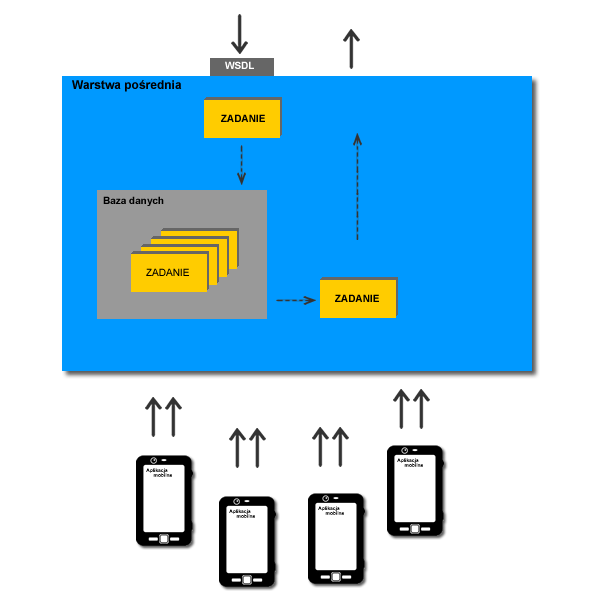
\includegraphics[scale=0.5]{middlewareTasksConceptDiagram}}
\caption{Poglądowy schemat wykorzystania zadań w warstwie pośredniej.}
\label{fig:middlewareTasksConceptDiagram}
\end{figure}

Na rysunku~\ref{fig:middlewareTasksConceptDiagram}. przedstawiono poglądowy schemat wykorzystania zadań w warstwie pośredniej. Strzałkami przerywanymi został oznaczony podstawowy cykl życia zadania. Po otrzymaniu żądanie od procesu BPEL warstwa pośrednia utworzy nowe zadanie i zapisze go w bazie danych. Aplikacje mobilne korzystając z lekkiego interfejsu komunikacyjnego, będą potrafiły pobierać zadania z bazy danych w celu ich rozwiązania. Po rozwiązaniu zadania, następować będzie wysłanie odpowiedzi do procesu biznesowego. 

\subsection{Dystrybucja zadań}
Przedstawiony powyżej schemat nie jest jednak kompletny. Oczywistym jest, że aby proces biznesowy miał sens powinien wykonywać więcej niż jedną operację, dla każdej operacji w proponowanym rozwiązaniu istnieć będzie zupełnie inna klasa zadań. Nie trudno dojść do wniosku, że każda z tych klas obsługiwana może być przez zupełnie różne grupy użytkowników. Na przykład niemal w każdym przedsiębiorstwie zadania dyrektora są kompletnie inne od zadań zwykłego pracownika, ale są one między sobą w jakiś sposób powiązane na przykład występują w tym samym procesie. Wnioskiem z tego płynącym jest konieczność wprowadzenia w warstwie pośredniej mechanizmu przydzielania zadań poszczególnym użytkownikom. W przypadku tym ponownie rozszerzenie \textit{BPEL4People} przewidziało ten problem i zaproponowało rozwiązanie. Wprowadza ono do każdej klasy zadań, definicje grupy docelowych adresatów. 

\begin{figure}[h]
\centerline{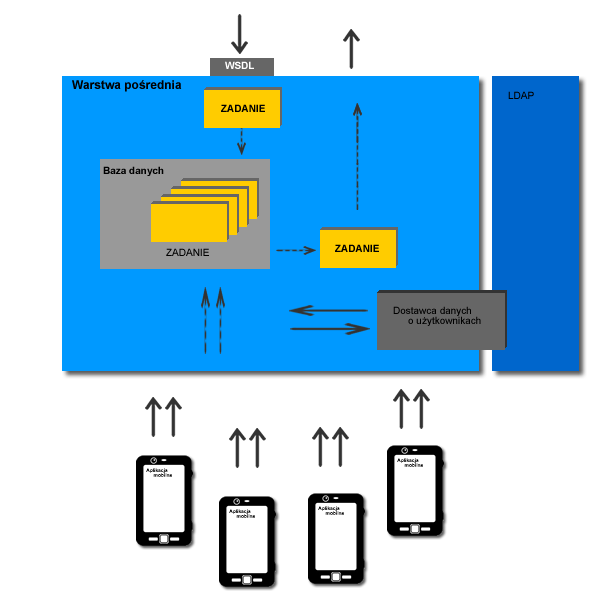
\includegraphics[scale=0.5]{middlewareUserDataProviderConceptDiagram}}
\caption{Schemat warstwy pośredniej uzupełniony o zarządzanie użytkownikami.}
\label{fig:middlewareUserDataProviderConceptDiagram}
\end{figure}

Na rysunku ~\ref{fig:middlewareUserDataProviderConceptDiagram} przedstawiono schemat warstwy pośredniej uzupełniony o zarządzanie użytkownikami. Aplikacje mobilne podczas rozwiązywania zadań będą przedstawiać się przy pomocy nazwy użytkownika. Przed pobraniem zadań z bazy danych dostawca danych o użytkownikach dostarczy informacji niezbędnych do określenia zadań specyficznych dla danego użytkownika. Sposób ten zapewni, że zadania należące do dyrektora przedsiębiorstwa nie trafią do zwykłych pracowników. 

Zastosowanie dodatkowej warstwy nazwanej \textit{Dostawcą danych o użytkownikach} jest tutaj celowe i będzie wymagać osobnej implementacji dla różnych rodzajów sposobów przechowywania danych o użytkownikach. Użytkownicy nie koniecznie muszą pochodzić z systemu katalogowego takiego jak LDAP. Możliwości przechowywania danych o użytkownikach jest bardzo wiele, dla prostych systemów lista użytkowników może być nawet predefiniowana.

\subsubsection{Context aware middleware}
Dodatkowym atutem udostępnienia możliwości implementacji dostawcy jest możliwość integracji adaptera z systemami zwanymi \textit{Context aware middleware}. 

\textit{Context aware middleware} jest oprogramowaniem które za pomocą danych dostarczanych z możliwie jak największej ilości źródł, stara się rozwiązać zadany problem. Rozwiązanie to bardzo szerokie zastosowanie znajduje głównie w aplikacjach mobilnych, dlatego że kontekst w przypadku tych aplikacji zmienia się bardzo dynamicznie. Architektura skupia się przede wszystkim na dostarczeniu informacji opisujących takie wymiary jak: - miejsce, Gdzie ? - czas, Kiedy? - stan np. Jaka jest temperatura otoczenia? - podmiot, Kto?

Bazując na tych danych stara się rozwiązywać dany problem w najbardziej optymalny sposób, na przykład przydzielając zadania osobie która jest najbliżej, która jest najmniej obciążona, która jest aktualnie w pracy itd.

Aby zastosować \textit{Context aware middleware} w warstwie pośredniej wystarczy odpowiednia implementacja dostawcy danych o użytkownikach. Uzyskamy dzięki takiemu rozwiązaniu potężne narzędzie potrafiące dystrybuować zadania w bardzo optymalny sposób zapewniając ich szybką realizację.  

\subsection{REST API}

Interfejs komunikacji warstwy pośredniej od strony procesów biznesowych został wymuszony przez specyfikację BPEL. Aby skompletować projekt warstwy pośredniej konieczne jest zdefiniowanie interfejsu komunikacyjnego od strony aplikacji mobilnych. 

Interfejs ten powinien przede wszystkim rozwiązywać podstawowy problem, występujący podczas rozwiązywania zadań przez wielu użytkowników jakim są konflikty. Nie może on dopuścić do sytuacji w której jedno zadanie byłoby rozwiązywanie przez wielu użytkowników jednocześnie. W celu rozwiązanie tego problemu konieczne jest wprowadzenie statusów zadań. W proponowanej warstwie pośredniej będą występowały następujące statusy zadania:

\begin{itemize}
\item gotowe do wykonania (ang. ready) -- zadanie zostanie oznaczone tym statusem tuż po utworzeniu. Użytkownik aplikacji mobilnych szukając zadań do wykonania otrzyma listę zadań oznaczonych właśnie tym statusem. 
\item przypisane (ang. climed) -- status ten oznacza, że któryś z użytkowników zadeklarował chęć jego wykonania. Będzie ono od tej pory dostępne tylko dla tego użytkownika. Pozostali użytkownicy poszukujący zadań do wykonania go nie zobaczą. 
\item rozwiązane (ang. completed) -- statusem tym oznaczone będą zadania zrealizowane z sukcesem, których rezultat został odesłany do procesu biznesowego. 
\item błąd podczas rozwiązywania (ang. failed) -- statusem tym oznaczone zostaną wszystkie zadania, podczas których rozwiązania wystąpił problem techniczny. 
\end{itemize}

Znając poszczególne statusy nadszedł czas na określenie interfejsu komunikacyjnego z aplikacjami mobilnymi. Ponieważ wśród aplikacji mobilnych najbardziej popularnym medium komunikacyjnym jest połączenie sieciowe na pewno najrozsądniejszym pomysłem będzie z niego skorzystanie. Jak wspomniano w rozdziale ~\ref{sec:analizaAplikacjiMobilnych}, podczas projektowania aplikacji mobilnych należy zwrócić uwagę na to aby wybierane technologie nie obciążały zbytnio ograniczonego pod względem zasobów urządzenia mobilnego. Dobrym wyborem w takim wypadku będzie REST. 

\subsubsection{Usługi sieciowe RESTFul}

REST (ang. Representational State Transfer) jest wzorcem narzucającym dobre praktyki tworzenia architektury aplikacji rozproszonych. Usługi sieciowe RESTFul  są usługami zaimplementowanymi na bazie protokołu HTTP i głównych zasad REST ~\cite{rest}.
Podstawą architektury REST jest zasób, zasób jest tutaj traktowany nie tylko jako jakiś byt, który można pobrać z aplikacji internetowej za pomocą protokołu HTTP. Zasobem w architekturze REST są również usługi udostępniane przez aplikacje internetowe.  

Kolejnym z głównych założeń architektury REST jest wykorzystanie metod udostępnianych przez protokół HTTP do definicji operacji wykonywanych na danym zasobie. Protokół HTTP oprócz najbardziej popularnych metod jak GET i POST udostępnia również całą gamę pozostałych metod. W architekturze REST oprócz tych dwóch najpopularniejszych bardzo często wykorzystywane są również PUT oraz DELETE. Znaczenie poszczególnych metod w kontekście operacji na zasobie może przedstawiać się następująco:
\begin{itemize}
\item GET -- pobranie danych
\item POST -- dodawanie danych
\item PUT -- edycja danych
\item DELETE -- usuwanie danych 
\end{itemize}


\subsubsection{Definicja interfejsu}

Warstwa pośrednia do komunikacji z aplikacjami mobilnymi będzie udostępniać następujące funkcje:

\begin{itemize}
\item lista zadań do wykonania -- metoda nie będzie przyjmować żadnych parametrów dodatkowych, kontekst użytkownika zostanie określony na podstawie nagłówków http wymaganych przez HTTP Basic Authentication. 
\item przypisz do zadania -- metoda jako parametr będzie przyjmować unikalny identyfikator zadania  
\item zrezygnuj z zadania -- metoda jako parametr będzie przyjmować unikalny identyfikator zadania  
\item rozwiąż zadanie -- metoda jako parametr będzie przyjmować unikalny identyfikator zadania  oraz wynik rozwiązania zadania. 
\end{itemize}

%---------------------------------------------------------------------------

\section{Wybrane technologie}
\label{sec:technologies}

Niemal w każdym projekcie informatycznym kluczową sprawą jest dobór odpowiednich technologii. Do realizacji warstwy pośredniej potrzebna będzie technologia webowa potrafiąca udostępnić usługi sieciowe, potrafiąca komunikować się z bazą danych i posiadająca wsparcie dla technologii REST. Niemal wszystkie popularne języki programowania spełniają każdy z tych warunków. Należy zatem pójść o jeden krok dalej i poszukać gotowego frameworka (zestawu gotowych bibliotek i wzorców postępowania), który przy wykorzystaniu jednego z tych języków będzie potrafił zrealizować przynajmniej cześć zadań. Wybór w niniejszej pracy magisterskiej padł na Spring Framework zaimplementowany w języku Java. 

\subsection{Spring Framework  }
Spring Framework zapewnia kompleksowy model programistyczny i konfiguracyjny dla nowoczesnych aplikacji biznesowych opartych na języku Java. Kluczowym elementem jest wsparcie infrastrukturalne  na poziomie aplikacji: Spring skupia się na "hydraulice" aplikacji dla przedsiębiorstw, tak, że zespoły mogą skupić się na logice biznesowej na poziomie aplikacji, bez konieczności określania środowisk programowania~\cite{springFramework}.

\begin{itemize}

\item Spring Web Services  -- w przypadku warstwy pośredniej jedną z głównych funkcjonalności koniecznych do realizacji jest udostępnienie usług sieciowych do komunikacji z procesami biznesowymi. Spring Framework posiada specjalnie do tego celu przygotowany moduł nazwany Spring Web Services. Moduł ten koncentruje się tworzeniu usług sieciowych na podstawie dokumentów SOAP przy wykorzystaniu stylu, umowa-najpierw(ang. contract-first). Styl ten polega na definicji interfejsów w postaci plików WSDL, przed stworzeniem konkretnej implementacji usługi. Jak argumentuje Spring styl ten pozwala na tworzenie elastycznych usług sieciowych przy wykorzystaniu jednego z wielu sposobów na manipulacje zawartością XML~\cite{springWS}.

\item Spring MVC -- moduł MVC jak sama nazwa wskazuje jest przeznaczony do tworzenia aplikacji opartych o jeden z najbardziej popularnych wzorców projektowych Model Widok Kontroler. Spring MVC jest przeznaczony przede wszystkim do zastosowania wzorca w aplikacjach webowych gdzie do komunikacji wykorzystywany jest protokół HTTP. W przypadku aplikacji webowych widokiem zazwyczaj jest dynamicznie generowany kod HML, nie jest to jednak reguła. W przypadku warstwy pośredniej MVC zostanie wykorzystane do przygotowania REST API. Widokiem w takim wypadku będą dane opisane za pomocą dokumentów JSON. 

\item Spring Data -- Oprócz wyżej wymienionych modułów, Spring Framework dostarcza również wsparcie do obsługi komunikacji z bazą danych, najczęściej do tego celu wykorzystując popularne ORM'y ( Biblioteki do mapowania obiektowo relacyjnego) jak Hibernate. W przypadku warstwy pośredniej istnieje konieczność przechowywania zadań w bazie danych dlatego Spring Data również zostanie wykorzystany.

\item Spring Secutiry -- W niniejszym rozwiązaniu uwierzytelnienia użytkowników REST API będzie odbywało się za pomocą HTTP Basic Authentication. Spring posiada również dodatkowe wsparcie do obsługi bezpieczeństwa przy pomocy HTTP Basic Authentication, wsparcie to udostępnione jest za pomocą modułu Spring Security.   

\end{itemize}

\subsection{MongoDB}

Bardzo ważną decyzją jest również wybór odpowiedniej bazy danych. Wymagania dotyczące warstwy pośredniej jasno określają, że głównym modelem przechowywanym w bazie danych będzie zadanie. Zadanie oprócz podstawowych informacji takich jak identyfikator, status, data utworzenia itd. będzie posiadał wszelkie informacje potrzebne do jego utworzenia, oraz jeśli zadanie zostanie wykonane posiadać będzie również informacje o rozwiązaniu. W przypadku skorzystania z relacyjnej bazy danych klaruje nam się przykładowy schemat bazy danych przedstawiony na rysunku ~\ref{fig:erd}.

\begin{figure}[h]
\centerline{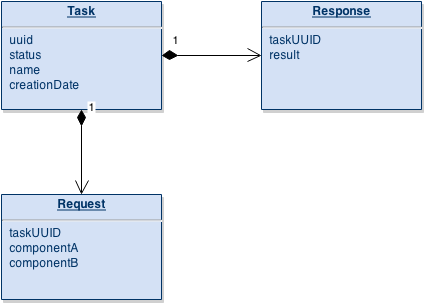
\includegraphics[scale=0.7]{erd}}
\caption{Diagram ERD przykładowego schematu bazy danych relacyjnej.}
\label{fig:erd}
\end{figure}

W przypadku pojedynczego zadania schemat może okazać się słuszny, problem powstaje gdy warstwa pośrednia obsługuje więcej niż jedno zadanie. W takim przypadku każdy kolejny rodzaj danych wejściowych poszczególnych zadań powinien znajdować się w osobnej tabeli. Mało tego dane wejściowe zadań nie muszą ograniczać się jedynie do płaskiej struktury danych. Mogą one zawierać argumenty będące osobnymi strukturami danych. W takich przypadkach, z punktu widzenia normalizacji bazy danych, każda z tych struktur powinna również znajdować się w osobnych tabelach.  Taka postać rzeczy ma bardzo negatywny wpływ na poziom komplikacji zapytań wyciągających zadania dla poszczególnych użytkowników. Mogą istnieć przypadki w których na podstawie danych wejściowych będzie potrzeba ograniczenia adresatów zadania, np. wybrania użytkowników w obrębie kilku kilometrów od adresu znajdującego się w danych wejściowych. 

Sposobem na rozwiązanie problemu nie koniecznie płaskiej struktury danych wejściowych może być zastosowanie typu XML do przechowywania tych danych. W takich przypadkach dane wejściowe zostałyby serializowane do dokumentów xml i w takiej postaci zapisane w bazie danych. Kolejny raz problemem są jednak skomplikowane zapytania do bazy danych. 

Odpowiedzią na postawione wymagania są dokumentowe bazy danych - w przypadku niniejszej pracy magisterskiej będzie to baza danych MongoDB ~\cite{mongodb}. Przechowują one dane w postaci kolekcji dokumentów. Dokumenty przechowywane w bazie danych mogą posiadać dowolnie skomplikowaną strukturę danych, a odpowiednio przygotowane zapytania będą potrafiły filtrować  listę tych dokumentów na podstawie wszystkich argumentów znajdujących się w tej strukturze. 

Przykładowy dokument bazy danych MongoDB może przedstawiać się następująco:

\begin{lstlisting}[caption=Zadanie w postaci dokumentu MongoDB.,numbers=left]
{	
	uuid : '6942cd9b-3b3b-49bd-9b18-de68384bd22a',
	name : 'createWarehouseDocument',
	state : '',
	createDate : '2014-07-24',
	priority: 3,
	request : {
		document :{
			type: 'inbound',
			company : {
				name : 'AGH',
				address : {
					city: 'Krakow',
					streat : 'al. A. Mickiewicza',
					number: '30',
					country: 'Polska'
				}
			},
			positions: [...]
		}
	}
}
\end{lstlisting}


Przedstawiony wyżej dokument jest przykładem zadania którego celem jest stworzenie odpowiedniego dokumentu magazynowego. Możemy sobie wyobrazić sytuację, że dokumenty dla kontrahentów z poszczególnych krajów są tworzone przez różnych użytkowników. Przykładowe zapytanie znajdujące wszystkie zadania dla użytkownika obsługującego Polskę wyglądało by następująco. 

\begin{lstlisting}[caption=Zapytanie MongoDB.]
{'request.document.company.address.country': 'Polska'}
\end{lstlisting}

W przypadku relacyjnej bazy danych powyższa struktura wymagała by stworzenie sześciu tabel a zapytanie które dałby by dokładnie taki sam rezultat wyglądało by następująco:

\begin{lstlisting}[caption=Zapytanie SQL.]
SELECT * FROM Tasks t 
	JOIN Request r ON t.id = r.task_id
	JOIN Document d ON r.id = d.request_id
	JOIN Company c ON d.id = c.document_id
	JOIN Address a ON c.id = a.company_id
WHERE a.country = 'Polska';
\end{lstlisting}

\subsection{Maven}
Kolejna technologią wykorzystaną do realizacji idei przestawionej w niniejszej pracy magisterskiej jest Maven. Wykorzystanie tej technologii wynika z decyzji wykorzystania języka Java. Maven jest narzędziem wspomagającym budowanie projektów stworzonych w języku Java. Odpowiada on za skompletowania wszystkich wymaganych bibliotek zdefiniowanych w odpowiednim pliku konfiguracyjnym - pom.xml. Biblioteki te pobierane są ze specjalnie przygotowanych do tego celu repozytoriów dostępnych w sieci, na lokalną maszynę. Biblioteki te są następnie wykorzystywane w procesie budowania plików wynikowych.  

%---------------------------------------------------------------------------

\section{Sprawienie rozwiązania generycznym}
\label{sec:generic}

Przedstawiony do tej pory model warstwy pośredniej skupia się przede wszystkim na problemie komunikacji pomiędzy procesem biznesowym oraz aplikacją mobilną, opisuje również sposób przechowywania i dystrybucji zadań. Model jest przy okazji bardzo ogólny i możliwy do zastosowania bez względu, na rozwiązywany problem. Nie ma w nim mowy o konkretnych przypadkach zastosowań. 

Dobrym pomysłem będzie więc stworzenie rozwiązania na tyle elastycznego aby mogło być wykorzystywane bez względu na rozwiązywany problem. W środowisku IT taki model postępowanie nazywany jest generycznym. W przypadku warstwy pośredniej sposób zarządzania zadaniami jest taki sam dla wszystkich rodzajów zadań - utworzenie zadania po otrzymaniu żądania od procesu, udostępnienie zadania aplikacją mobilnym, odpowiedź do procesu. Główną różnicą są dane wejściowe różnych żądań oraz sposób dystrybucji zadań pomiędzy aplikacjami na podstawie tych danych. Problem różnych struktur danych wejściowych dla różnych zadań rozwiązuje nam wybór bazy danych MognoDB, który będzie potrafił zapisać te struktury bez dodatkowych konfiguracji, oraz będzie potrafił je przeszukiwać za pomocą prostych zapytań. 

Problem różnego sposobu dystrybucji danych rozwiążemy za pomocą pliku konfiguracyjnego, który będzie opisywał poszczególne zadania, oraz definiował jakie grupy użytkowników są uprawnione do ich rozwiązywania.

Opisany model można zobrazować za pomocą schematu widocznego na rysunku ~\ref{fig:middlewareGenericConcept}.

\begin{figure}[h]
\centerline{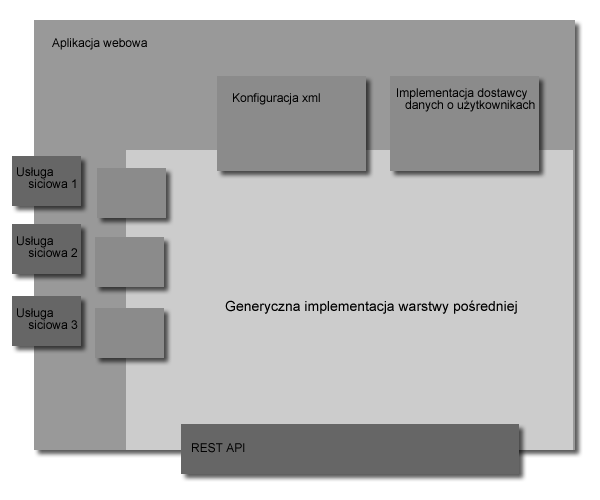
\includegraphics[scale=0.6]{middlewareGenericConcept}}
\caption{Poglądowy schemat wydzielenia biblioteki odpowiedzialnej za obsługę warstwy pośredniej.}
\label{fig:middlewareGenericConcept}
\end{figure}

Podsumowując, opisane w niniejszej pracy magisterskiej rozwiązanie będzie generyczną biblioteka służącą do tworzenie aplikacji webowej. Aplikacja ta będzie warstwa pośrednią pomiędzy procesem biznesowym a aplikacjami mobilnymi. 

%---------------------------------------------------------------------------

\section{Implementacja}
\label{sec:impl}

Implementacja biblioteki zostanie przedstawiona w sposób schematyczny, zostanie przedstawiony projekt klas występujących w rozwiązaniu wraz z ich opisem. W następnej część zostaną przedstawione diagramy sekwencji najważniejszych funkcjonalności rozwiązania, opisujące przebieg wywołań kolejnych funkcji zdefiniowanych klas. 

\subsection{Diagram klas}

\begin{figure}[h]
\centerline{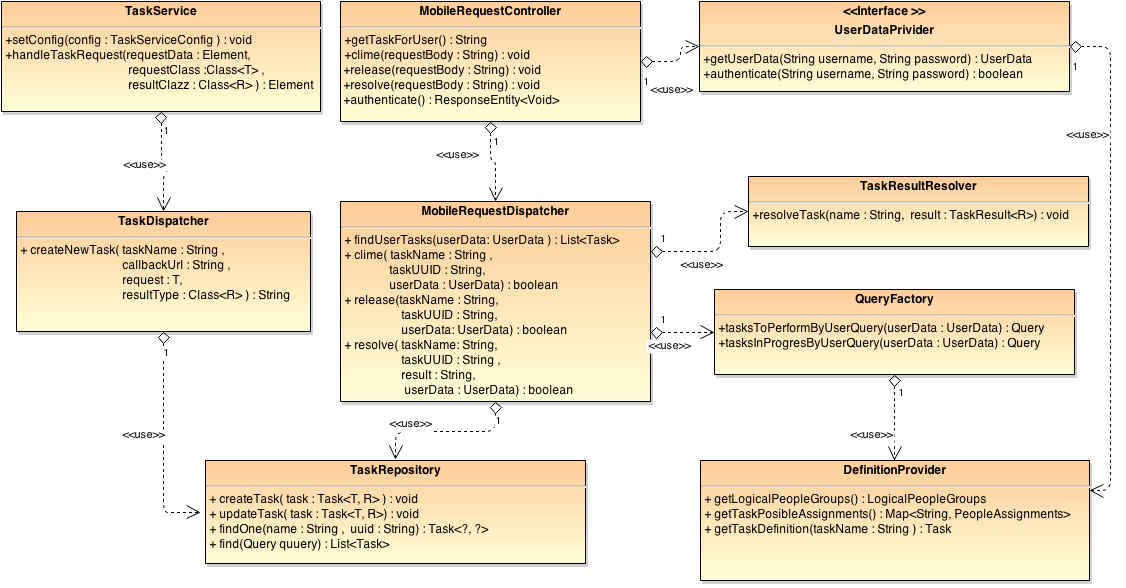
\includegraphics[scale=0.45]{classDiagram}}
\caption{Diagram klas implementacji warstwy pośredniej.}
\label{fig:classDiagram}
\end{figure}

Diagram klas przedstawiony na rysunku~\ref{fig:classDiagram}. przedstawia zestaw klas, które wymagają dodatkowego objaśnienia: 


\begin{itemize}
\item TaskService -- jest to klasa odpowiedzialna za obsługę żądań pochodzących z procesów biznesowych. Każdy rodzaj zadania powinien posiadać własną instancję tej klasy, która z kolei powinna być wykorzystywana przez usługę sieciową odpowiedzialną za jego obsługę. Klasa posiada dwie metody, setConfig odpowiedzialną za ustawienie podstawowych informacji o zadaniu, które będzie obsługiwać instancja tej klasy, takich jak nazwa, lista klas definiujących dane wejściowe i wyjściowe zadania. Kolejną metodą jest metoda handleTaskRequest metoda ta przyjmuje jako parametr obiekt typu Element zawierający dane wejściowe w postaci XML. Metoda przetwarza te dane na odpowiednie klasy i zapisuje zadanie w bazie danych do późniejszej realizacji. Zwraca ona obiekt typu Element zawierający informacje o unikalnym identyfikatorze przypisanym zadaniu, obiekt ten jest plikiem xml który powinna zwrócić usługa sieciowa. Metoda handleTaskRequest powinna zostać wywołana przez usługę sieciową odbierającą żądanie od procesu biznesowego.
\item TaskDispatcher -- Klasa odpowiedzialna za przetwarzanie, przyjętych przez klasę TaskService zadań. Posiada ona jedną metoda służącą do zapisu zadania przetworzonego przez  TaskService, nazwaną createNewTask.
\item TaskRepository -- repozytorium zadań odpowiedzialne za obsługę bazy danych. Posiada metody służące do zapisu i edycji zadań oraz do wyszukiwania zarówno pojedynczych zadań, jak i ich listy. 
\item MobileRequestController -- klasa przeznaczona do udostępnienia REST API. Posiada ona metody udostępniane przez interfejs przeznaczony do aplikacji mobilnych. Klasa ta korzystając ze Spring Security, odnajduje kontekst aktualnego użytkownika, pobiera informacje o nim za pomocą UserDataProvidera przekazując następnie kontrole MobileRequestPrivider'owi. 
\item UserDataProvider -- interfejs służący do określenia metod które musi implementować dostawca informacji o użytkowniku. Implementacje UserDataProvidera będą wykorzystywana między innymi przez Spring Security.
\item DefinitionProvider -- klasa to odpowiedzialna jest za deserializację pliku xml zawierającego konfiguracje poszczególnych zadań, oraz dostarczenie tej konfiguracji do pozostałych klas warstwy pośredniej. 
\item MobileRequestDispatcher -- klasa odpowiedzialna za obsługę żądaniami pochodzącymi z aplikacji mobilnych. Współpracuje z klasami przeznaczonymi do generowania zapytań, wyciągania danych z bazy oraz odpowiedzialnymi za odesłanie rozwiązania do procesów biznesowych. 
\item QueryFactory -- głównym zadaniem tej klasy jest przygotowanie zapytań pozwalających odnaleźć zadania dostępne dla danego użytkownika. Zapytania generowane są na podstawie konfiguracji xml oraz danych o użytkowniku. 
\item TaskResultResolver -- klasa posiada tylko jedną metodę nazwaną resolveTask służąca do wysłania odpowiedzi do procesu biznesowego zawierającej rezultat wykonania zadania. 
\end{itemize}

\subsection{Diagramy sekwencji}

Sposób działania powyżej opisanych klas zostanie przedstawiony za pomocą diagramów sekwencji. Diagramy przedstawiają sekwencje kolejnych wywołań funkcji w celu realizacji funkcjonalności dostarczanych przez warstwę pośrednią. 

\begin{figure}[h]
\centerline{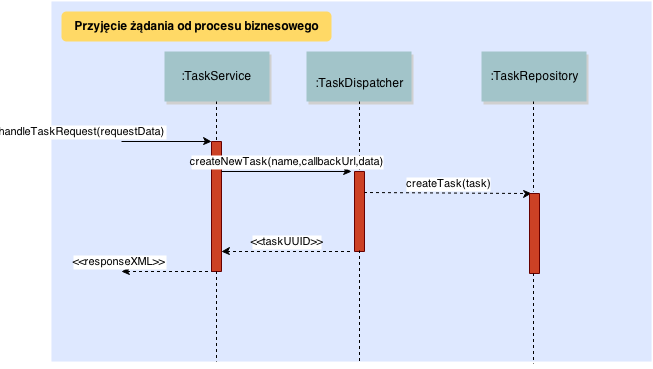
\includegraphics[scale=0.6]{createTaskFlow}}
\caption{Diagram sekwencji obsługi żądania pochodzącego z procesu BPEL.}
\label{fig:createTaskFlow}
\end{figure}

Na rysunku~\ref{fig:createTaskFlow} zobaczyć można diagram sekwencji funkcjonalności -przyjęcie żądania od procesu biznesowego. Usługa sieciowa korzystając z konkretnej instancji klasy TaskService uruchamia metodę handleTaskRequest przekazując do niej obiekt zawierający dokument XML z danymi wejściowymi. Wewnątrz metody, dokument XML zostaje zdeserializowany do postaci obiektów podanych w konfiguracji klasy TaskService. Zostaje również wydobyty adres url usługi przyjmującej ostateczny rezultat zadania. Sterowanie przekazywane jest następnie do klasy TaskDispatcher w celu utworzenie nowego zadania w bazie danych. Metoda createNewTask klasy TaskDispatcher oprócz stworzenia nowego dokumentu w kolekcji w bazie danych MongoDB za pomocą repozytorium TaskRepository, odpowiedzialna jest za generację unikalnego identyfikatora w postaci klucza GUID. Unikalny identyfikator jest następnie zwracany ponownie do TaskService'u gdzie zostaje opakowany w dokument XML, który zostanie zwrócony do procesu biznesowego. Wysłanie unikalnego klucza do procesu jest w tym przypadku krytyczne, po stronie silnika uruchomieniowego procesów biznesowych BPEL będzie istniało bardzo wiele instancji procesów w różnym stadium wykonania. Komunikacja procesu z warstwą pośrednią odbywa się w sposób asynchroniczny, poprzez kolejne wywołania aktywności request (wysłanie żądania), by następnie przejść do aktywności recieve (oczekiwać na jego rezultat). W między czasie proces może również wykonać inne operacje. Aby skojarzyć aktywność wysłania żądania z otrzymaniem żądania w przypadku wielu instancji procesu konieczna jest identyfikacja tych żądań za pomocą tego samego unikalnego klucza. W procesach biznesowych BPEL mechanizm ten został nazwanych mechanizmem korelacji.  Aby skorzystać zatem z mechanizmy korelacji, podczas tworzenia nowego zadania proces biznesowy musi otrzymać unikalny klucz tego zadania by następnie podczas otrzymania rezultatu zadania był w stanie skojarzyć ten rezultat z konkretną instancją procesu. Rezultat w takim wypadku również musi zostać podpisany unikalnym identyfikatorem zadania. 

\begin{figure}[h]
\centerline{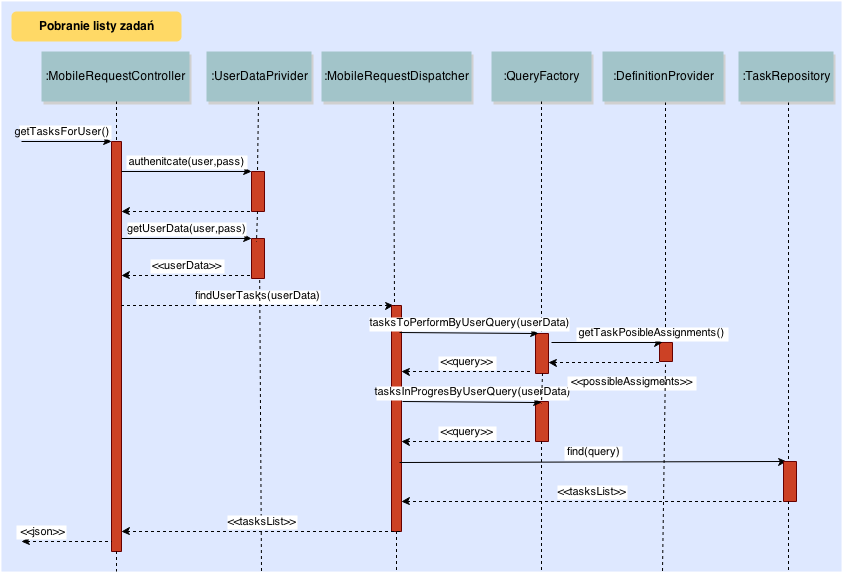
\includegraphics[scale=0.5]{tasksListFlow}}
\caption{Diagram sekwencji pobrania listy zadań dostępnych dla użytkownika.}
\label{fig:tasksListFlow}
\end{figure}

Rysunek~\ref{fig:tasksListFlow} przedstawia diagram sekwencji pobierania listy zadań przez aplikację mobilną. Sekwencja w tym przypadku zaczyna się od klasy MobileRequestController, która jest odpowiedzialna za obsługę żądań odpowiednich żądań http. Kontroler ten rozpoczyna wykonanie metody od autentykacji użytkownika którym przedstawia się żądanie http (z wykorzystaniem http basic authentication). Po poprawnej autentykacji zostają pobrane informacje o aktualnym użytkowniku, informacje te zostaną wykorzystane do wygenerowania listy zadań dla niego dostępnych.  Sterowanie zostaje następnie przekazane do klasy MobileRequestDispatcher, która za pomocą QueryFactory zbuduje dwa zapytania, jedno do wyciągnięcia nowych zadań do których użytkownika ma dostęp. Drugie zapytanie pokryje wszystkie zadania w trakcie realizacji przypisane do użytkownika. Zapytania te posłużą następnie do wyciągnięcia listy zadań z bazy danych przy pomocy repozytorium TaskRepository. Ostatnim krokiem będzie serializacja wydobytych zadań do postaci dokumentu JSON. 

\begin{figure}[h]
\centerline{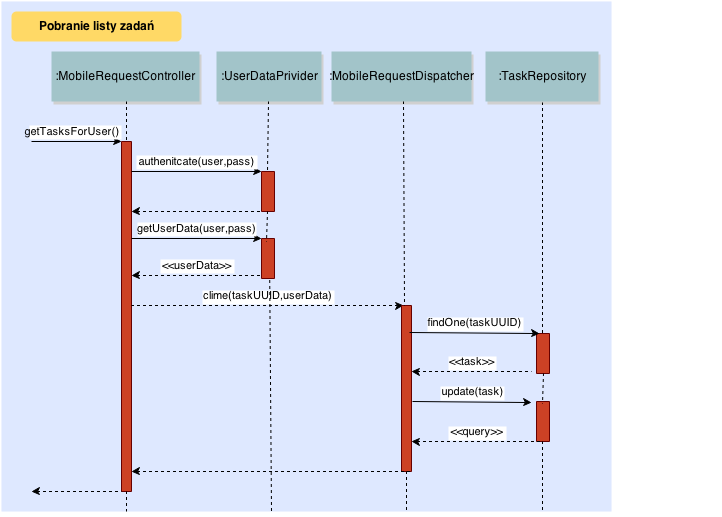
\includegraphics[scale=0.5]{climeTaskFlow}}
\caption{Diagram sekwencji przypisania użytkownika do zadania.}
\label{fig:climeTaskFlow}
\end{figure}

Rysunek ~\ref{fig:climeTaskFlow} przedstawia diagram przypisania konkretnego zadania do użytkownika. Przypisanie odbywa się za pomocą REST API. Odpowiednie żądanie HTTP zostaje przyjęte przez MobileRequestController, ponownie jak w przypadku pobierania listy zadań, dwie pierwsze operacje wykonywane przez kontroler to autentykacja i pobranie informacji o użytkowniku. Sterowanie zostaje następnie przekazane do MobileRquestDispatcher'a, który znajduje odpowiednie zadanie w repozytorium, zmienia jego status uzupełniając informacje o przypisanym użytkowniku by następnie zapisać te zmiany. Operacją kompensacyjną do przypisania jest operacja zwolnienia zadania. Diagram sekwencji w przypadku tej drugiej wygląda niemal identycznie jak diagram przypisania z tym że MobileRequrestDispatcher przywraca zadaniu status do realizacji. 

\begin{figure}[h]
\centerline{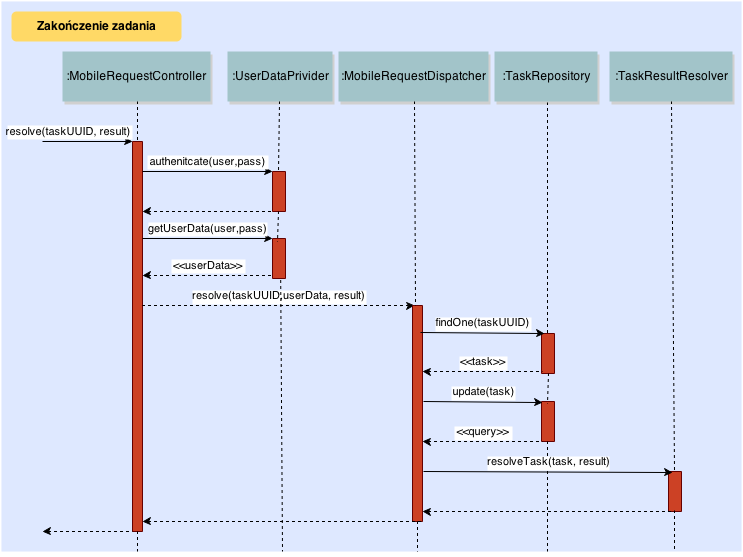
\includegraphics[scale=0.5]{resolveTaskFlow}}
\caption{Diagram sekwencji rozwiązania zadania.}
\label{fig:resolveTaskFlow}
\end{figure}

Na rysunku ~\ref{fig:resolveTaskFlow} przedstawiono ostatni rodzaj funkcjonalności jakim jest obsługa rozwiązania zadania. Decyzja o rozwiązaniu również pochodzi od strony aplikacji mobilnej i a funkcjonalność ją obsługująca udostępniona jest za pomocą REST API. Tak jak w poprzednich przypadkach przed rozpoczęciem przetwarzania żądania następuje autentykacja oraz pobranie informacji o użytkowniku. Następnie pobierane zostaje zadanie z repozytorium, ustawiany rezultat oraz zmieniany status. Rezultat następnie zostaje odesłany do procesu biznesowego przez klasę TaskResultResolver. Jeśli odesłanie rezultatu zakończy się sukcesem zadanie z odpowiednio ustawionym statusem i rezultatem zostaje zapisane do bazy danych.


%---------------------------------------------------------------------------

%\section{Notyfikacje}
%\label{sec:notifications}

%// TODO
